%%%%%%%%%%%%%%%%%%%%%%%%%%%%%%%%%%%%%%%%%
% University/School Laboratory Report
% LaTeX Template
% Version 3.1 (25/3/14)
%
% This template has been downloaded from:
% http://www.LaTeXTemplates.com
%
% Original author:
% Linux and Unix Users Group at Virginia Tech Wiki 
% (https://vtluug.org/wiki/Example_LaTeX_chem_lab_report)
%
% License:
% CC BY-NC-SA 3.0 (http://creativecommons.org/licenses/by-nc-sa/3.0/)
%
%%%%%%%%%%%%%%%%%%%%%%%%%%%%%%%%%%%%%%%%%

%----------------------------------------------------------------------------------------
%	PACKAGES AND DOCUMENT CONFIGURATIONS
%----------------------------------------------------------------------------------------

\documentclass{article}

\usepackage[version=3]{mhchem} % Package for chemical equation typesetting
\usepackage{siunitx} % Provides the \SI{}{} and \si{} command for typesetting SI units
\usepackage{graphicx} % Required for the inclusion of images
\usepackage{natbib} % Required to change bibliography style to APA
\usepackage{amsmath} % Required for some math elements 
\usepackage[nodayofweek,level]{datetime}
\usepackage{mdframed}
\usepackage{listings}
\usepackage{enumitem}
\usepackage{grffile}

\lstset{ %
language=C,                    % choose the language of the code
basicstyle=\footnotesize,         % the size of the fonts that are used for the line-numbers
breaklines=true,
postbreak=\raisebox{0ex}[0ex][0ex]{\ensuremath{\color{red}\hookrightarrow\space}}
}

\setlength\parindent{0pt} % Removes all indentation from paragraphs

%\usepackage{times} % Uncomment to use the Times New Roman font

%----------------------------------------------------------------------------------------
%	DOCUMENT INFORMATION
%----------------------------------------------------------------------------------------

\title{Exploring Wireshark \\ CEEN 8886 --- Wireless Security} % Title

\author{Kelly \textsc{Boswell} \\ krboswell@gmail.com} % Author name

\date{\Large March 27, 2017} % Date for the report

\begin{document}

\maketitle % Insert the title, author and date

\begin{center}
\begin{tabular}{l r}
Date Performed: & March 25, 2017 \\ % Date the experiment was performed
Instructor: & Professor Yi Qian % Instructor/supervisor
\end{tabular}
\end{center}

% If you wish to include an abstract, uncomment the lines below
% \begin{abstract}
% Abstract text
% \end{abstract}

%----------------------------------------------------------------------------------------
%	SECTION 1
%----------------------------------------------------------------------------------------

\section{Objective}

The objectives for this lab experiment are as follows:

% If you have more than one objective, uncomment the below:
\begin{itemize}
\item Learn to read WEP authentication traffic using Wireshark
\item Record home network's traffic and explore home networking environment
\end{itemize}

%----------------------------------------------------------------------------------------
%	SECTION 2
%----------------------------------------------------------------------------------------

\section{Requirements}

Some prerequisites for completing this lab experiment are as follows:

\begin{itemize}
\item A laptop or desktop equipped with a functioning wireless adapter supporting
      802.11 modules
\item Wireshark network analyzer
\end{itemize}

%----------------------------------------------------------------------------------------
%	SECTION 3
%----------------------------------------------------------------------------------------

\section{Experiment Steps And Results}

\begin{enumerate}
\item \label{step1} Downloaded and opened the provided PCAP (lab2.pcap) file. The file may be
                    downloaded from the course website. This file contains a full 802.11 authentication
                    session.
    \begin{enumerate}
        \item \label{1a} Before unrolling any packets, identified the SSID information of the WAP. The
              SSID is ``DENVEROFFICE''. See Figure \ref{fig:step1a}. There are two packets that contain
              this SSID and they are packets 1 and 10. 
        \item \label{1b} Unrolled packet 1 and identified the destination MAC address. See Figure
               \ref{fig:step1b}. Beacon frames are broadcasted periodically to announce the presence of
               the wireless LAN and devices with compatible wireless LAN adapters may be made known of
               their presence.  This is why the broadcast destination (ff:ff:ff:ff:ff:ff) is used.
        \item \label{1c} Unrolled packet 4 and identified the source and destination MAC addresses.
               See Figure \ref{fig:step1c}. In this packet, the WAP is the source of the transmission.
        \item \label{1d} Unrolled packet 6 and identified the decoded WEP password. See Figure
              \ref{fig:step1d}.
        \item \label{1e} Unrolled packet 8 and found evidence that the WEP authentication was successful.
    \end{enumerate}
\item \label{step2} Explore home networking environment.
    \begin{enumerate}
        \item \label{2a} Started up a computer in my home network and connected to the internet via a wireless
              interface.
        \item \label{2b} Launched a web browser and started playing a long YouTube video.
        \item \label{2c} Started up wireshark and began capturing traffic on the wireless interface.
        \item \label{2d} Stopped capturing traffic after a short interval (I think I accidentally
              captured far more than just 15 seconds of data) and saved the capture as
              Lab3-KRB.pcapng.gz (gzipped PCAP-NG).
        \item \label{2e} During this brief interval, 10342 packets were captured. See Figure
              \ref{fig:step2e}.
        \item \label{2f} All of the protocols contained in this capture are: ARP, DHCP, DNS, ICMPv6,
              IGMPv2, LLMNR, MDNS, NBNS, QUIC, SSDP, TCP, TiVoConnect, and UDP.
        \item \label{2g} My MAC Address is f0:7d:68:c1:b3:c2 and my LAN IP address is 192.168.1.10. See
              Figure \ref{fig:step2g}.
        \item \label{2h} No 802.11 protocol packets were captured, therefore no SSID information could be
              found in the overall capture.

    \end{enumerate}
\end{enumerate}

\begin{figure}
\begin{mdframed}
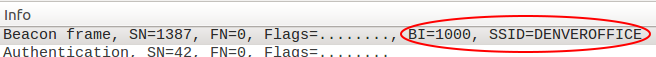
\includegraphics[scale=0.5]{Step_1a.png}
\caption{Identifying the SSID information of the WAP.}
\label{fig:step1a}
\end{mdframed}
\end{figure}

\begin{figure}
\begin{mdframed}
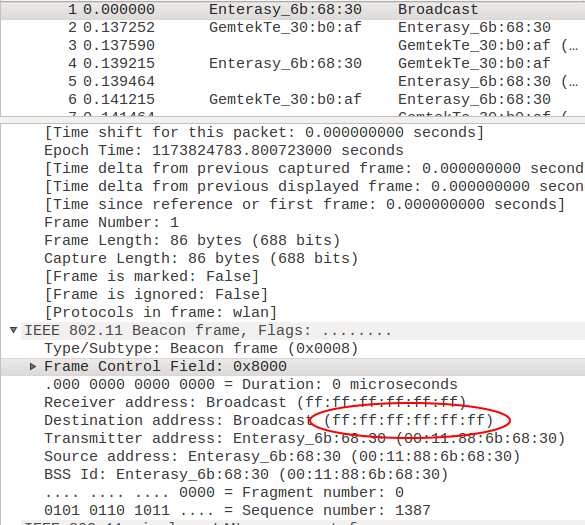
\includegraphics[scale=0.5]{Step_1b.png}
\caption{Identifying the destination MAC in packet 1.}
\label{fig:step1b}
\end{mdframed}
\end{figure}

\begin{figure}
\begin{mdframed}
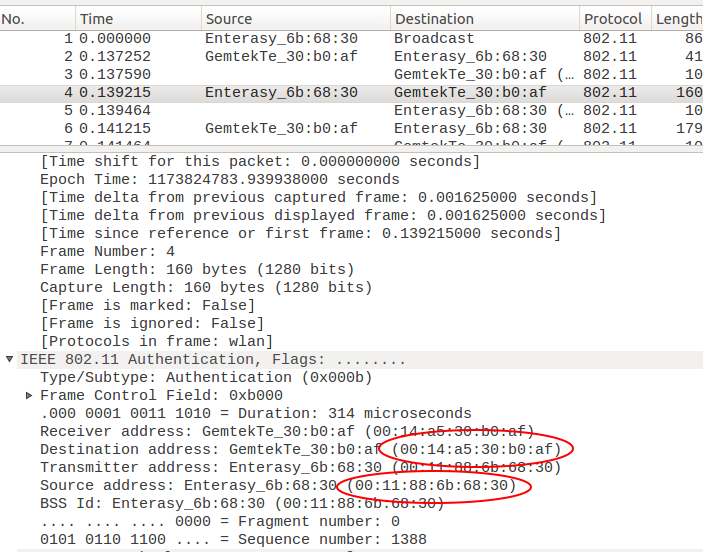
\includegraphics[scale=0.4]{Step_1c.png}
\caption{Identifying the source and destination MAC in packet 4.}
\label{fig:step1c}
\end{mdframed}
\end{figure}

\begin{figure}
\begin{mdframed}
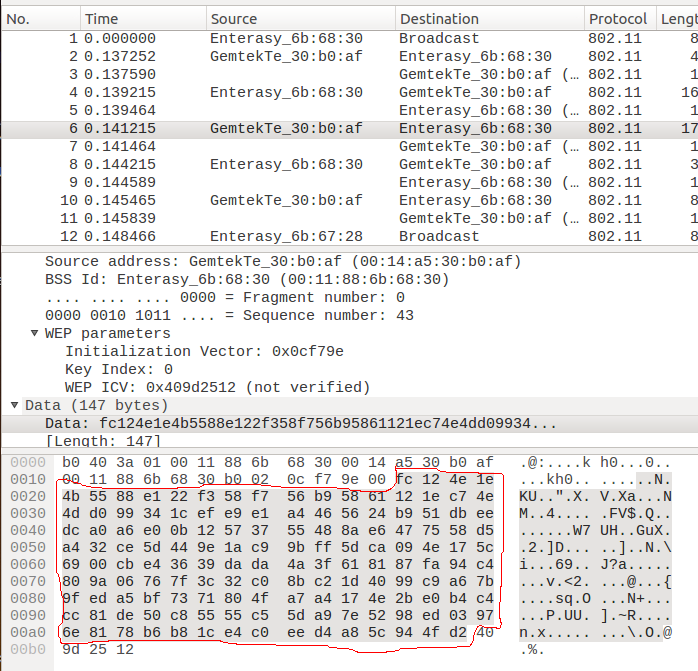
\includegraphics[scale=0.4]{Step_1d.png}
\caption{Identifying the decoded WEP password in packet 6.}
\label{fig:step1d}
\end{mdframed}
\end{figure}

\begin{figure}
\begin{mdframed}
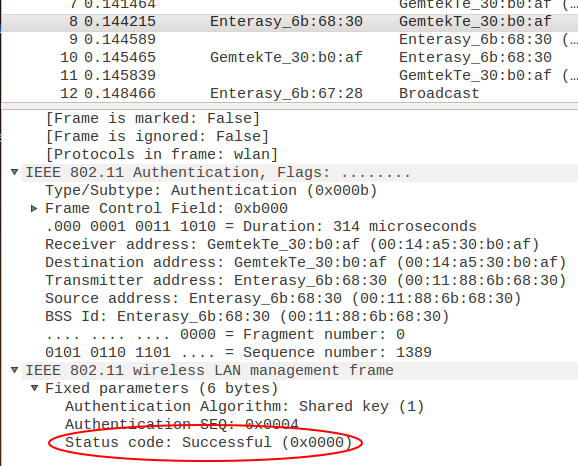
\includegraphics[scale=0.5]{Step_1e.png}
\caption{Finding evidence that WEP authentication succeeded in packet 8.}
\label{fig:step1e}
\end{mdframed}
\end{figure}

\begin{figure}
\begin{mdframed}
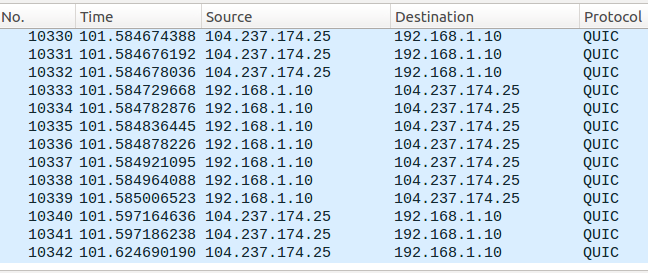
\includegraphics[scale=0.5]{Step_2e.png}
\caption{Screenshot of home network capture.}
\label{fig:step2e}
\end{mdframed}
\end{figure}

\begin{figure}
\begin{mdframed}
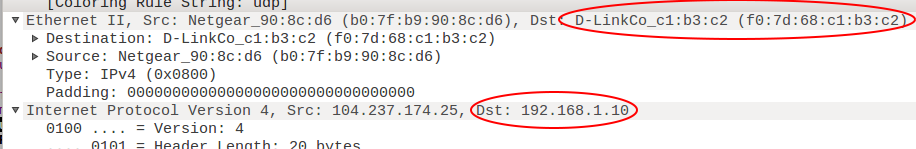
\includegraphics[scale=0.35]{Step_2g.png}
\caption{Screenshot of MAC and LAN IP.}
\label{fig:step2g}
\end{mdframed}
\end{figure}

%----------------------------------------------------------------------------------------
%	SECTION 4
%----------------------------------------------------------------------------------------

\end{document}
